\section{Methodology}
\label{sec:method}

%%----------------------------------------------------------------
%% Overview Figure
%%----------------------------------------------------------------
\begin{figure*}[t]
	\begin{center}
	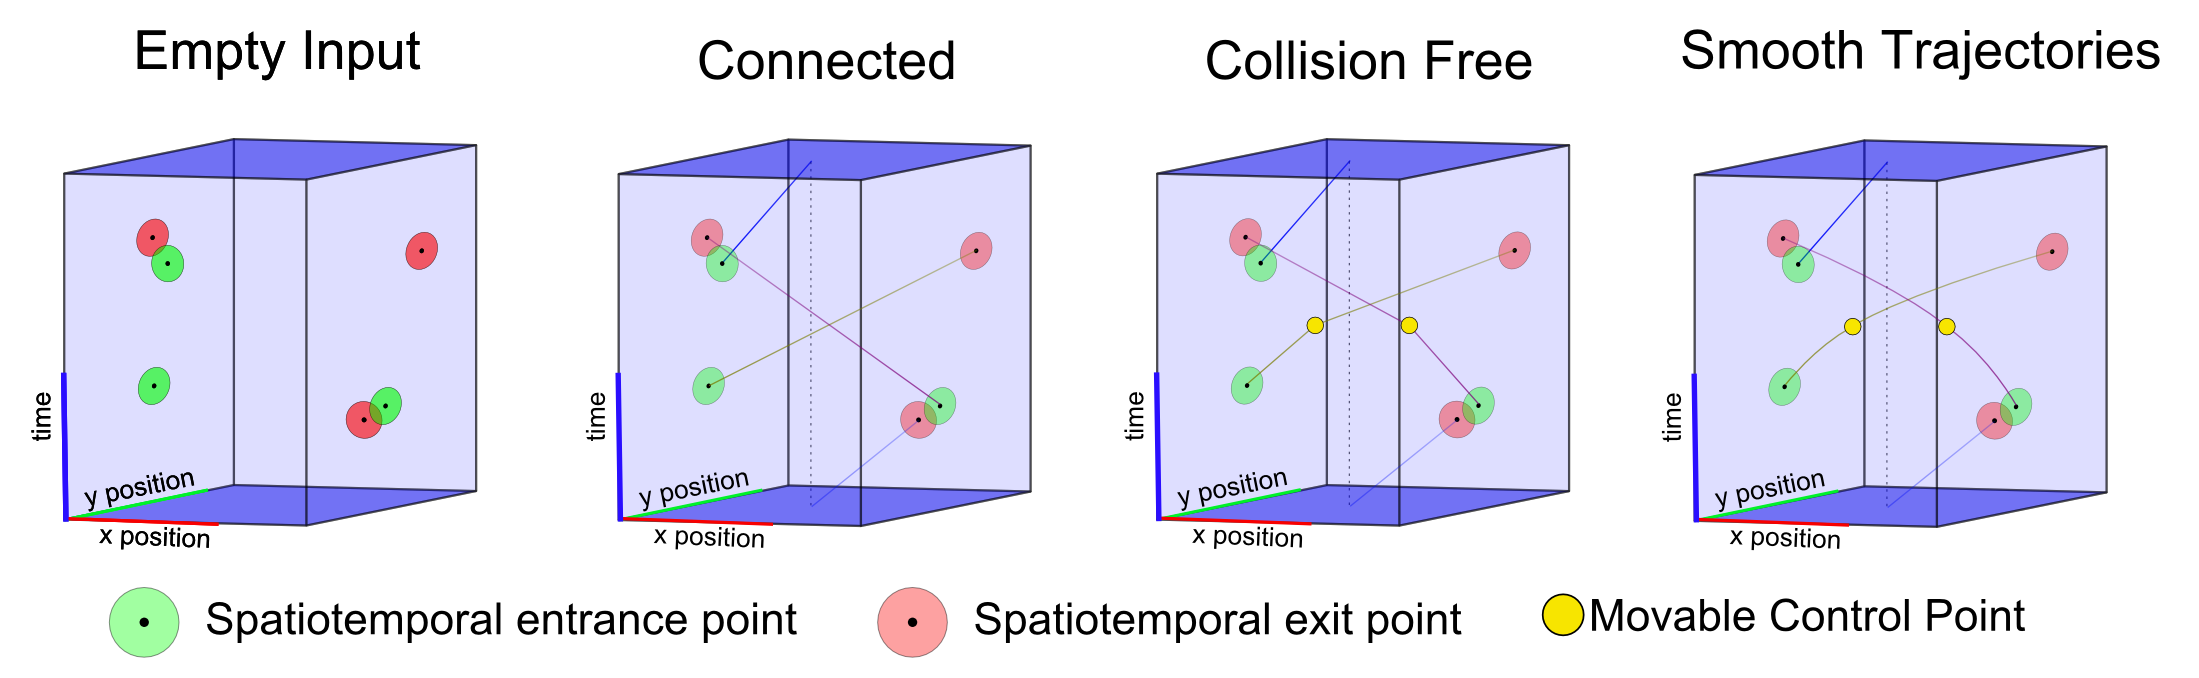
\includegraphics[width=0.9\linewidth]{./images/overview-hd.png}
% 	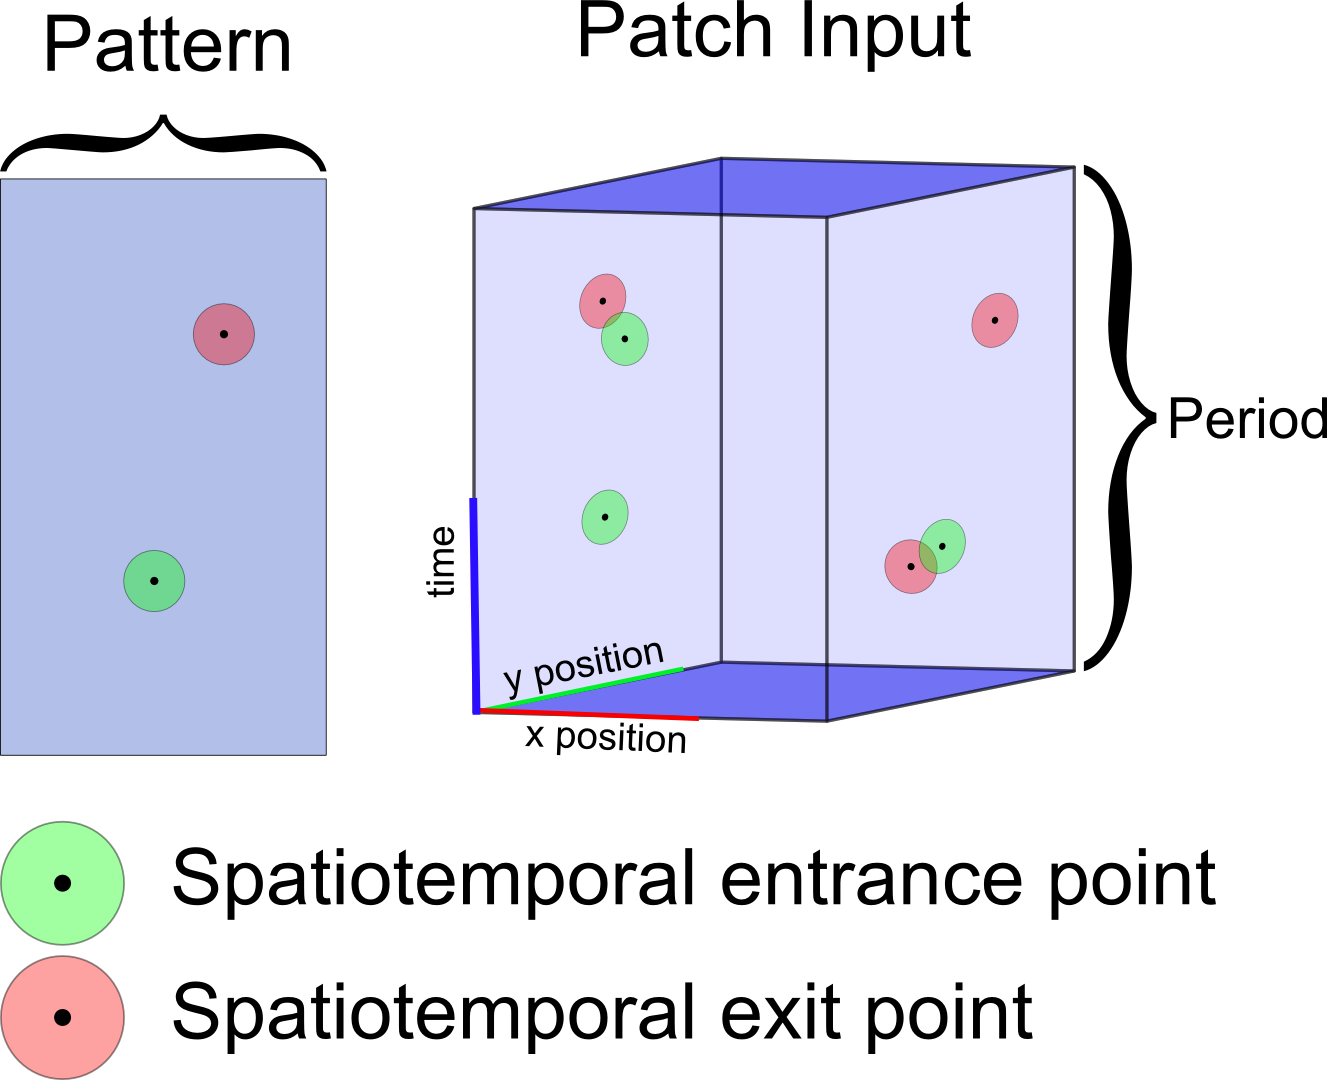
\includegraphics[height=4cm]{./images/patches-empty-patch-with-pattern.png}
% 	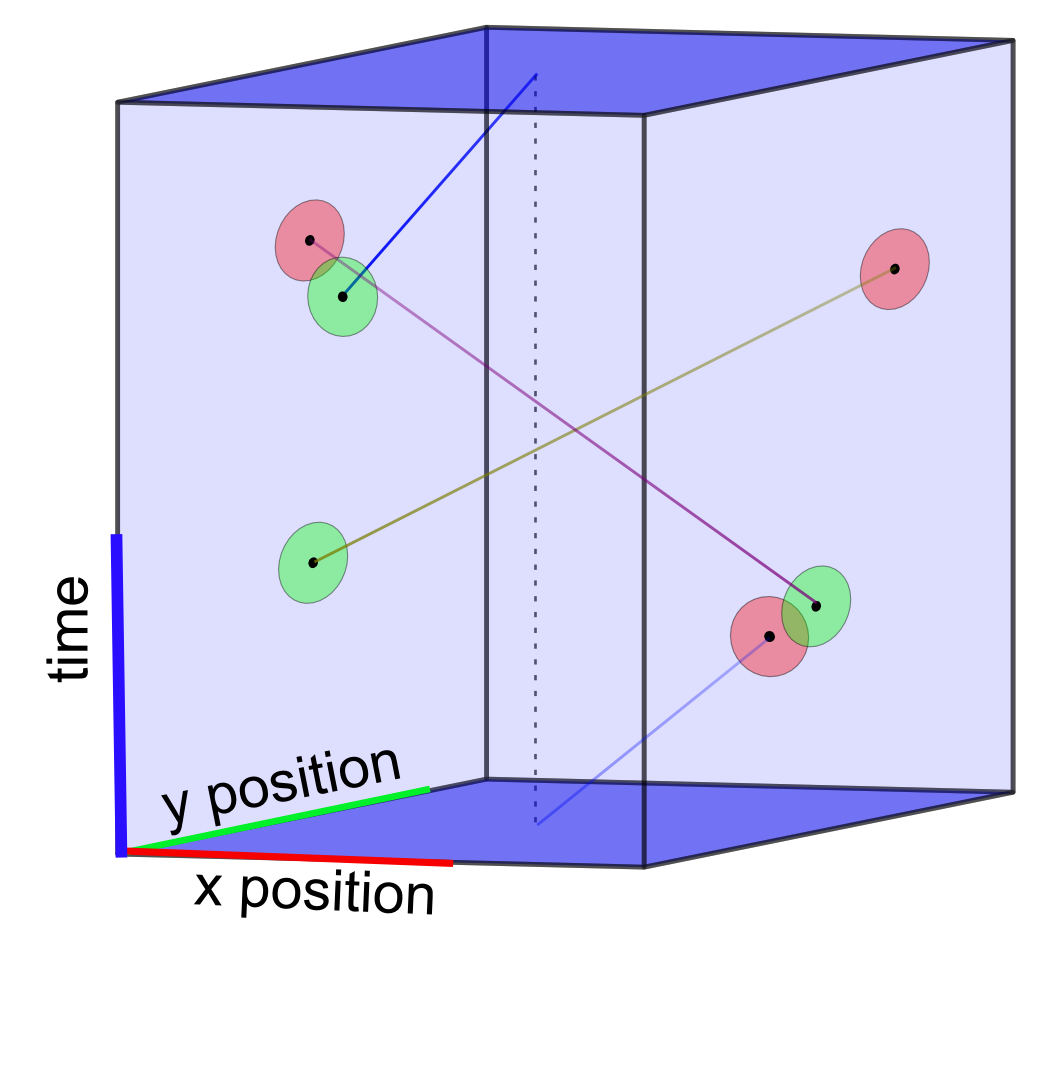
\includegraphics[height=4cm]{./images/patches-connected-patch.png}
% 	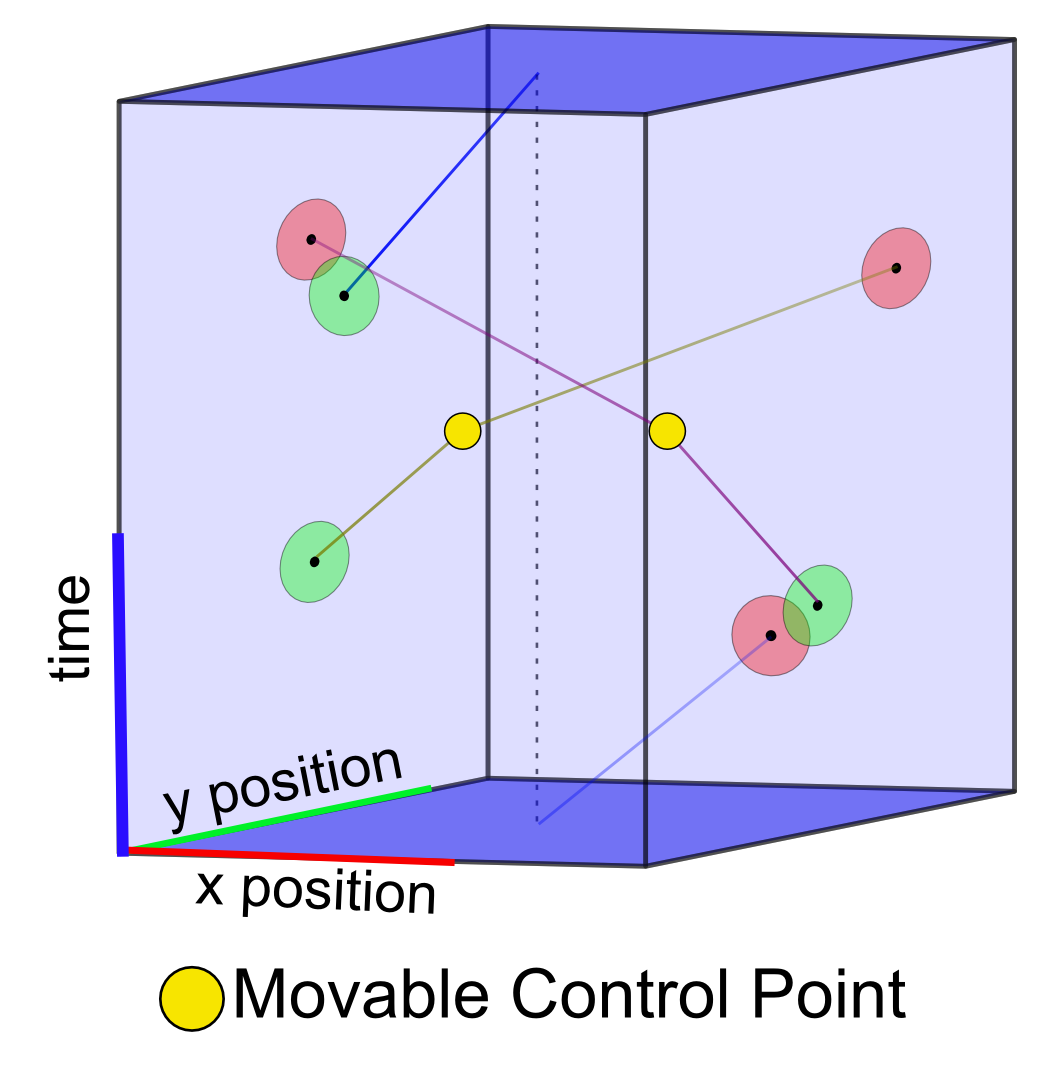
\includegraphics[height=4cm]{./images/patches-collision-free-patch.png}
% 	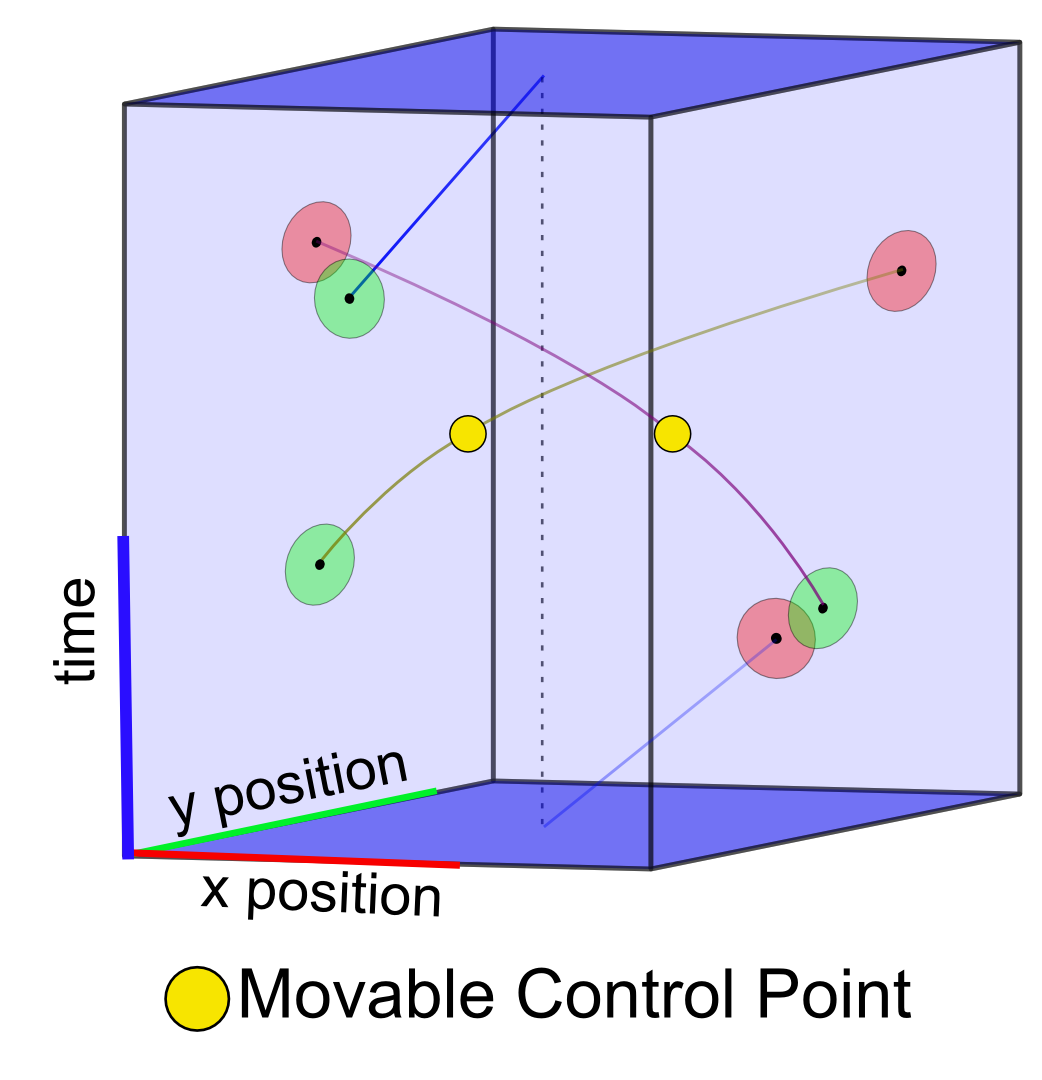
\includegraphics[height=4cm]{./images/patches-smoothed-patch.png}
	\caption{
		\textbf{Overview} Input and output points in a patch's patterns are initially connected and subsequently modified and smoothed out to be collision free.
	}
	\label{fig:overview}
	\end{center}
\end{figure*}
%%----------------------------------------------------------------
%% Overview Figure
%%----------------------------------------------------------------

\note{Overview: remind definitions on crowd patches: patch, pattern, spatiotemporal waypoints (boundary conditions: input, output, initial states // boundary conditions should be strictly enforced. Movable control points), period of time \dots}

\note{Starting Definitions:}

\begin{description}

\item[Patch]{
A patch is a set $\{ A, \pi, D, S\}$ where $A$ is a geometrical area with a convex polygonal shape, $\pi$ the period of time of the animation and $D$ and $S$ are the sets of dynamic and static objects, respectively.
These last two sets may be empty in case of an empty patch.
}

\item[Static obstacles]{
Static objects are simple obstacles whose geometry is fully contained inside the patch.
}

\item[Dynamic objects]{
Dynamic objects are animated; i.e., they are moving in time according to a set of trajectories $T$.
}

\end{description}

We define a {\bf trajectory} inside a patch as a function going from time to position, more specifically from the subset $[ 0,\pi ]$ to $A$:$ \tau:[t_1,t_2]\rightarrow A, \hspace{0.3cm} 0 \leq t_1 < t_2 \leq \pi$.
We represent a trajectory as a list of control points connected by segments. 
\note{THIS I A LITTLE BIT CONFUSING}

A {\bf control point} is a point in space and time $\mathbf{cp} = \{\mathbf{a}_{cp}, t_{cp}\}$. All control points in a trajectory can either be boundary or movable ones. Boundary control points serve as entry and exit points to the patch and cannot be moved, added or deleted. Movable control points can be moved, added, or removed from the trajectory as long as they do not violate the constraints of the patch; i.e., their positions $\mathbf{a}_{cp}$ must lie inside area $A$ and their time $t_{cp}$ must be between $t_1$ and $t_2$.

A {\bf segment} is a straight line connecting two control points in a specific order. Since these are unidirectional lines in space-time, it is important to remember that they are not allowed to go backwards in time.

There are two categories of dynamic objects: endogenous and exogenous agents. {\bf Endogenous agents} remain inside $A$ for the total period of time $\pi$. In order to achieve periodicity for the animation, they are associated with a trajectory $\tau : [0,\pi] \leftarrow A$, such that it respects the periodicity condition: the position at the start and at the end of the animation must be the same, i.e. \mbox{$\tau (0) = \tau (\pi)$}.\\
{\bf Exogenous agents} go outside $A$. They enter the patch at time $t_{initial}$ and position $a_{initial}$, and they exit at time $t_{final}$ and position $a_{final}$. For each agent we associate a sequence of $n \ge 1$ trajectories $\{ \tau_1, \tau_2, \dots, \tau_n\}$. Sequences may have only one trajectory, but some agents require additional trajectories in order to satisfy speed and time constraints. The following conditions must be respected in each sequence of trajectories associated with an exogenous agent:

\begin{itemize}

\item{$a_{initial}$ and $a_{final}$ must be points in the border of $A$. Otherwise, they couldn't be exogenous agents.}

\item{If the sequence is composed by more than one trajectory, for each two contiguous trajectories, the following must be true to ensure continuity: $\tau_i(\pi) = \tau_{i_{next}}(0)$.}

\end{itemize}

Note that the second condition implicitly implies that in sequences with multiple trajectories, each middle trajectory must be fully defined in the period of time $[0,\pi]$, while $\tau_1$ must be defined in $[t_{initial},\pi]$ and $\tau_n$ must be defined in $[0, t_{final}]$.

\begin{description}

\item[Pattern -]{If a patch is a spatio-temporal cube (or any other right prism, depending on the type of polygon used as its area, then a pattern could be defined as one lateral side of the \note{cube (or right prism).} Specifically, it is a rectangle whose base is one of the edges of the polygonal area (we define $I$ as this two dimensional vector), and its height is equal to the period. These patterns also include the sets of boundary control points. We divide this set evenly into two subsets: Input and Output. The Input set contains the boundary control points where exogenous agents begin their trajectories; we call these Entry Points. Conversely the elements of Output are called Exit Points. They establish the position in time and space that the exogenous agents finish their paths. Formally defined, a patch P is:
$$ P = {l, p_i, I_i [p_i, t_i], O_j[p_j, t_j]}$$
We populate virtual environments by sticking patches together. Thus, we have to ensure continuity between trajectories for exogenous agents passing through two contiguous patches. This means that two adjacent patches must \note{have a similar pattern on the side they share}. The vector $l$ \claudia{Is this vector $l$ or $I$?, please check } and period must be equivalent and the sets of Input and Output are exchanged. If we have $P_1={l, pi, I [p_1,t_1], O[p_2,t_2]}$ and $P_2={l�, pi�, I�[p�_2, t�_2], O�[p�_1, t�_1]}$, then, in order to satisfy $C^0$ continuity we must ensure: 
$$ l=l�, pi=pi�, p_1=p�_1, t_1=t�_1, p_2=p�_2, t_2=t�_2.$$
We then say $P_1$ is the mirror pattern of $P_2$. In the animation, this will be seen as an agent going from one patch to an adjacent one. 
If the area of a patch is a square, the patch defines 4 patterns, one for each of its sides. Patterns defined by a patch have the property that the sum of the cardinality of all the Inputs is the same as the sum of the cardinality of all Outputs. We call this the parity condition: $\sum(|Inputs|)= \sum(|Outputs|)$.

A patch defines a set of Patterns, and conversely, a set of patterns satisfying the parity condition, having the same period, and whose vectors define a convez polygonal area, can be used to create a patch. 
 }

\end{description}

\subsection{Overview}
\label{method:overview}

The objective is, given a set of patterns, we want to construct a patch.
This process has three main steps:
\begin{enumerate}
  \item Make a matching between the elements in the Input and Output sets contained within a patch. In this step, we connect Entry to Exit Points based on a scoring function. This function tries to keep agents close to their prefered speed while at the same time avoiding connections to similar patterns, thus reducing unwanted u-turns.  The input for this function is a set of patterns and the output is a set of piecewise linear trajectories connecting the entry and exit points.
  \item Create collision free trajectories for these pairings. We start with simple line trajectories and start bending them until they are collision free. Points lying at the borders, i.e. the Entry and Exit points, are hard restraints and can never be moved.
  \item Smoothing trajectories (if needed).  Last, we use splines to minimize the hard turns. We make sure the new trajectories stay close to the original ones, lest we create new collisions.
\end{enumerate}

\note{Problem : is to compute internal trajectories that join all boundary conditions with conitnuous and believable motion trajectories. 

2 steps: 
 - step 1: connect waypoints
INPUT first boudnary conditions are ``alone'' in patches $\rightarrow$ associate/connect waypoints
 them 
OUTPUT : initial trajectories (piecewise linear trajs, possibly colliding, with ``good'' properties that we will define later on)

 - step 2: optimize intial trajectories by moving control points to remove collisions
    INPUIT : initial trazjectories
      OUTPUT : colliision trajectories, still enforcing boundary conditions
      
- step 3 is smoothing
}       


\subsection{Connecting Boundary Control Points}

The first step to this algorithm is to match all the entry and exit points.  To do this, we have to measure how good or bad a match is. Intuitively, there are some better matches than others, Judging by sight, trajectories passing near the center of the patch look better that the ones staying close to the borders. We can consider some other aspects too, like how close the speed needed for the agent to go from the Entry Point to the Exit Point is to comfort speed. We use a comfort speed of $1.33~m/s$ which is the normal walking speed of humans in an unconstrained environment.

For a square patch, we prefer to match points with points on the opposite pattern. Then the points on the contiguous pattern and finally, the points that are in the same pattern. If there are multiple options on the same pattern we choose the point whose associated trajectory is closest to comfort speed.

To solve this matching problem, we make use of the Gale-Shapley algorithm~\cite{gale1962college} (see Algorithm~\ref{alg:stable-matching}), commonly referred to as the algorithm to solve the stable marriage problem.  This algorithm assures that at the end, if we have Alice engaged to Bob and Carol engaged to Dave, it is not possible for Alice to prefer Dave and Dave to prefer Alice. We call that a stable matching.  

This pseudocode demonstrates the Gale-Shapley algorithm in relation to two equal lists of men and women who are being matched for marriage. However the algorithm generalizes to any matchable objects, which in our case is entry and exit points.

%%-------------------------------------------------------------------
%% The Stable Matching Algorithm by Gale-Shapley
%%-------------------------------------------------------------------
\begin{algorithm}[t]
Put here the algorith of stablematching
\caption{Stable Matching Algorithm}
\label{alg:stable-matching}
\end{algorithm}
%%-------------------------------------------------------------------
%% The Stable Matching Algorithm by Gale-Shapley
%%-------------------------------------------------------------------


All we need in order to use this algorithm is a to generate preferences for entry and exit points. We do this with the following steps:
\begin{enumerate}
  \item Find the speed it would take to travel from an Entry Point to an Exit Point.  Let�s assume $(p_1, t_1)$ is position and time of the Entry Point and $(p_2,t_2)$ the equivalent of the Exit point. Speed is $d/t$ where $d=|p_1-p_2|$ and $time=t_2-t_1$ in case $t_2>t_1$. Otherwise, $time=period+t_2-t_1$. More details on why we take this time will be given later when we create the initial set of trajectories.
  \item Now, we assign each pair of points a number between $0$ and $\pi/2$, where $0$ represents maximum closeness to comfort speed with $arctan(|comfort speed -speed|)$.
  \item We add penalties for points being in the same patch, for those points, we add $4$. For points lying in the contiguous pattern we also add a smaller penalty, $2$.
  \item We sort each list.
\end{enumerate}
\panayiotis{The steps above need editing}    
 
We will have a list similar to this for each entry and exit point, we call this list the proposal list:
